\section{RA en Android}
\frame
{
\frametitle{¿Qué opciones hay?}
{\setlength{\arrayrulewidth}{0mm}
\begin{table}[ht]
  \centering
  \begin{tabular}{| m{3cm} | m{4cm} | m{4cm} |}
  \hline
  
\includegraphics[height=2cm, width=1.8cm]{imgs/opencv.png} & 
     \hspace{2cm}
\includegraphics[width=3cm]{imgs/vuforia.png} & 
     \hspace{2cm}
\includegraphics[width=3cm]{imgs/metaio.jpg}
  \end{tabular}
\end{table}
}

{\setlength{\arrayrulewidth}{0mm}
\begin{table}[ht]
  \centering
  \begin{tabular}{| m{4cm} | m{4cm} |}
  \hline
  
\includegraphics[width=2cm]{imgs/layar.jpg}& 
\includegraphics[width=2cm]{imgs/wikitude.png}
  \end{tabular}
\end{table}
}
}

\subsection*{OpenCV}
\frame
{
\frametitle{OpenCV for Android}
\begin{itemize}
 \item Biblioteca libre de \textbf{visión artificial} originalmente desarrollada por \textbf{Intel}
 \item En 2008, la empresa \textbf{Willow Garage} asume el soporte. En 2012, lo hace la empresa \textbf{ItSeez}.
 \item Disponible para Windows, Linux, Mac, Android e iOS
 \item Para Android se proporciona la API Java con clases específicas, que es un subconjunto de la API de C
 \item SDK Quick start\\ \url{http://docs.opencv.org/doc/tutorials/introduction/android_binary_package/O4A_SDK.html}
 \item Utilizado en aeronaves no tripuladas, sistemas de vigilancia, reconocimiento facial, etc.
\end{itemize}
}

\frame
{
\frametitle{OpenCV for Android: ventajas e inconvenientes}
\begin{itemize}
\item \textbf{Ventajas:}
  \begin{itemize}
   \item Licencia BSD
   \item Buen rendimiento
   \item Multiplataforma
   \item Soporte de la comunidad. Multitud de snippets.
  \end{itemize}

\item \textbf{Inconvenientes:}
  \begin{itemize}
   \item La API de Java es un subconjunto mínimo. Para obtener un conjunto mayor, se recomienda usar el NDK + JNI. Más info: \\
     \url{http://www.nacho-alvarez.es/index.php/blog/2012/05/02/conectar-programas-cc-con-aplicaciones-android/}
   \item El sobreimpresionado de elementos debe hacerse manualmente
   \item Se centra en visión por computador, así que no tenemos la parte GPS
   \item Hace falta una formación específica en visión artificial para utilizarla correctamente
  \end{itemize}

\end{itemize}
}

\frame
{
\frametitle{OpenCV for Android: recursos}
\begin{itemize}
\item \textbf{OpenCV4Android:} \url{http://opencv.org/platforms/android.html}
\item \textbf{Quick Start:} \url{http://docs.opencv.org/doc/tutorials/introduction/android_binary_package/O4A_SDK.html}
\item \textbf{Android development with OpenCV:} \url{http://docs.opencv.org/doc/tutorials/introduction/android_binary_package/dev_with_OCV_on_Android.html}
\item \textbf{Java API:} \url{http://docs.opencv.org/java/}
\end{itemize}
}

\subsection*{Vuforia}
\frame
{
\frametitle{Vuforia}
\begin{itemize}
 \item Biblioteca que permite reconocer y hacer el seguimiento de imágenes planas (Image Targets) y objetos 3D simples
 \item Desarrollo de Qualcomm Austria Research Center Gmbh
 \item Disponible para Android, iOS y Unity
 \item Incluye la parte NDK + JNI pre-compilada. Sólo tenemos que incluir las bibliotecas y llamar a los métodos nativos.
 \item Targets disponibles: Image, Cylinder, Text-Word, User-defined, Cloud Recognition, Multi-Targets, Frame markers y Virtual buttons.
\end{itemize}
}

\frame
{
\frametitle{Vuforia: Cloud Recognition}
 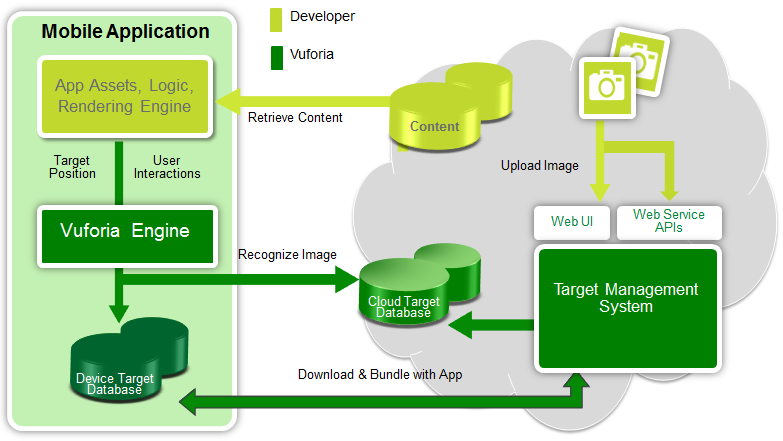
\includegraphics[width=12cm]{imgs/vuforia-components.png}
}

\frame
{
\frametitle{Vuforia: ventajas e inconvenientes}
\begin{itemize}
\item \textbf{Ventajas:}
  \begin{itemize}
   \item Licencia QTL: gratuito y puede usarse en apps comerciales
   \item Gran rendimiento
   \item Posibilidad de reconocimiento en la nube
   \item Clases más sencillas que en OpenCV
  \end{itemize}

\item \textbf{Inconvenientes:}
  \begin{itemize}
   \item Dependencia de NDK + JNI. Si se quiere ampliar, se amplían los métodos nativos.
   \item Cloud recognition no es totalmente gratuito y no podemos montar nuestro propio server
   \item Se centra en visión por computador, así que no tenemos la parte GPS
   \item Foro de debate, con menor orientación a comunidad
  \end{itemize}

\end{itemize}
}

\frame
{
\frametitle{Vuforia: recursos}
\begin{itemize}
\item \textbf{Descarga SDK:} \url{https://developer.vuforia.com/resources/sdk/android}
\item \textbf{Instalación SDK:} \\\url{https://developer.vuforia.com/resources/dev-guide/step-2-installing-vuforia-sdk}
\item \textbf{Target Manager:} \url{https://developer.vuforia.com/targetmanager/project/checkDeviceProjectsCreated?dataRequestedForUserId=}
\item \textbf{Sample apps:} \url{https://developer.vuforia.com/resources/sample-apps}
\end{itemize}
}

\subsection*{Metaio}
\frame
{
\frametitle{Metaio}
\begin{itemize}
 \item Fundado en 2003 en Munich por Thomas Alt y Peter Meier
 \item Se estructura en \textit{canales}
 \item Ofrecen un conjunto de productos:
 \begin{itemize}
   \item \textbf{metaio SDK + metaio Cloud:} SDK de desarrollo para metaio con cuenta de acceso a Cloud. 
   \item \textbf{metaio Creator + metaio Cloud:} aplicación de escritorio para crear AR channels y visualizarlo en junaio.
   \item \textbf{junaio:} navegador de realidad aumentada.
 \end{itemize}
 \item Disponible para Android, iOS y Windows
\end{itemize}
}

\frame
{
\frametitle{Junaio: ventajas e inconvenientes}
\begin{itemize}
\item \textbf{Ventajas:}
  \begin{itemize}
   \item Posibilidad de reconocimiento en la nube
   \item Posibilidad de montar tu propia nube
   \item SDK muy sencillo y bien documentado
   \item Buen soporte orientado a comunidad de desarrolladores
  \end{itemize}

\item \textbf{Inconvenientes:}
  \begin{itemize}
   \item Pequeño lag a veces
   \item Eliminar la marca de agua es caro
   \item No es libre
   \item La plataforma web es demasiado compleja 
  \end{itemize}

\end{itemize}
}
